\documentclass[a4paper, fontsize=10pt, DIV=9, parskip=half, headings=small]{scrartcl}
%
\usepackage{ifluatex}
\usepackage[ngerman]{babel}
%
\ifluatex
 % LuaLaTeX
 \usepackage{fontspec}
 \usepackage{selnolig}
\else
 % PdfLaTeX
 \usepackage[T1]{fontenc}
\fi
%
\usepackage{csquotes}
\usepackage{microtype}
%
\usepackage{graphicx}
%
\usepackage[headsepline, footsepline=false]{scrlayer-scrpage}
\pagestyle{scrheadings}
\clearpairofpagestyles
%
\ihead{BV1 Übungsblatt 3}
\chead{Jonas Pardeyke \& Nik Tykhomyrov, \today}
\ohead{\pagemark}
%
\usepackage{lastpage}
%
\renewcommand*\pagemark{{\usekomafont{pagenumber}{\pagename~\thepage\,/\,3}}}
%
\title{BV1 – Übungsblatt 3 \\ \large Schriftliche Ausarbeitung}
\author{Jonas Pardeyke \& Nik Tykhomyrov}
\date{\today}

\usepackage[utf8]{inputenc}
\usepackage{graphicx}
\usepackage{amsmath}
\usepackage{hyperref}
\usepackage{caption}
\usepackage{float}

%------------------------------------------------------------------------------
%
\begin{document}

\maketitle 

\section{Einleitung}

Im Rahmen der Veranstaltung Bildverarbeitung 1 (BV1) befasst sich dieses Übungsblatt mit verschiedenen Verfahren zur Binarisierung von Grauwertbildern. Die Aufgabe beinhaltet die Implementierung des Otsu-Verfahrens, die Recherche und den Vergleich mit adaptiven Schwellenwertverfahren sowie die Anwendung von Morphologie zur Rauschreduktion und abschließend der Einsatz von Masken zur Bildkombination.

Ziel ist es, die Unterschiede der Verfahren praktisch zu erfahren, ihre Wirksamkeit anhand konkreter Beispiele zu beurteilen und typische Nachbearbeitungsschritte wie Erosion und Dilatation gezielt einzusetzen. Diese Prozesse sind in vielen Anwendungen der Bildverarbeitung essenziell, etwa in der Objekterkennung, Dokumentanalyse oder medizinischen Bildauswertung.

\section{Hauptteil}

\subsection{Aufgabe 1: Otsu-Verfahren}

Das Otsu-Verfahren dient der automatischen Bestimmung eines binären Schwellenwerts, indem die Varianz zwischen Klassen maximiert wird. Ich habe das Verfahren in Python mit NumPy implementiert und auf verschiedene Grauwertbilder angewendet.

Der binäre Schwellenwert wurde anschließend genutzt, um das Bild in zwei Klassen zu unterteilen. Die Ergebnisse wurden mit der OpenCV-Implementierung
\texttt{cv2.threshold(img, 0, 255, cv2.THRESH\_BINARY + cv2.THRESH\_OTSU)} verglichen. Die resultierenden binären Bilder waren qualitativ nahezu identisch, minimale Unterschiede zeigten sich lediglich durch Rundungsfehler.

\begin{figure}[H]
  \centering
  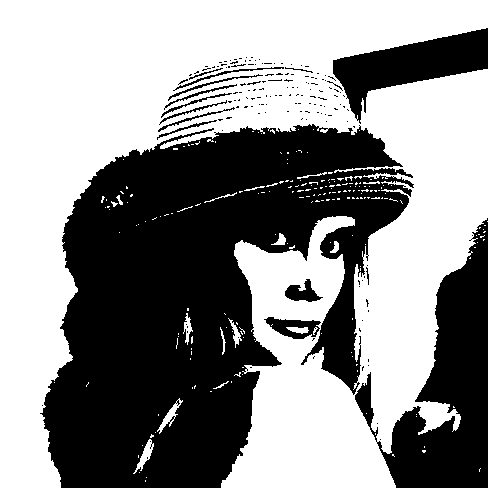
\includegraphics[width=0.4\textwidth]{otsu_custom.png}
  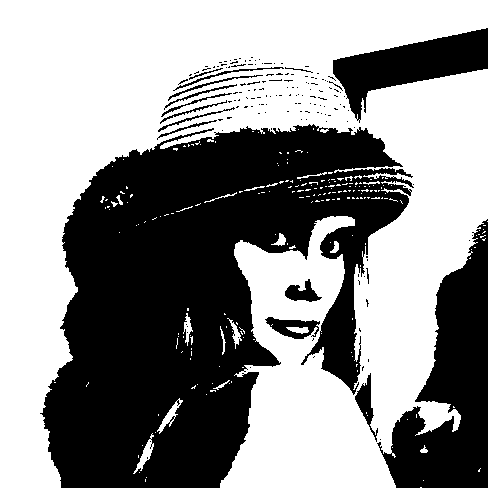
\includegraphics[width=0.4\textwidth]{otsu_opencv.png}
  \caption{Links: eigene Implementierung, Rechts: OpenCV}
\end{figure}

\subsection{Aufgabe 2: Adaptive Thresholding (cv.ADAPTIVE\_THRESH\_GAUSSIAN\_C)}

Im Gegensatz zu Otsu berücksichtigt das adaptive Thresholding lokale Bildregionen, was insbesondere bei ungleichmäßiger Beleuchtung Vorteile bietet. Mit
\texttt{cv2.adaptiveThreshold()} und der Option \texttt{cv2.ADAPTIVE\_THRESH\_GAUSSIAN\_C} wurden deutlich differenziertere Ergebnisse erzielt – feine Details blieben besser erhalten.

\begin{figure}[H]
  \centering
  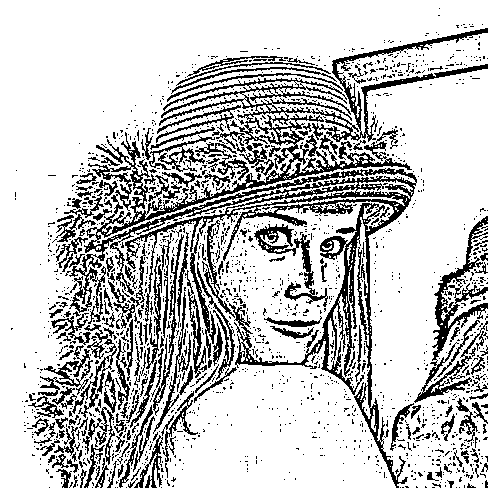
\includegraphics[width=0.4\textwidth]{adaptive_thresh.png}
  \caption{Ergebnis mit cv.ADAPTIVE\_THRESH\_GAUSSIAN\_C}
\end{figure}

\subsection{Aufgabe 3: Rauschentfernung mit Morphologie}

Ein besonders verrauschtes Bild wurde gezielt ausgewählt. Nach der binären Schwellenwertbildung waren viele isolierte weiße Pixel sichtbar. Durch Anwendung von
\texttt{cv2.erode()} gefolgt von \texttt{cv2.dilate()} (Opening) konnte das Rauschen signifikant reduziert werden, ohne relevante Strukturen zu zerstören.

\begin{figure}[H]
  \centering
  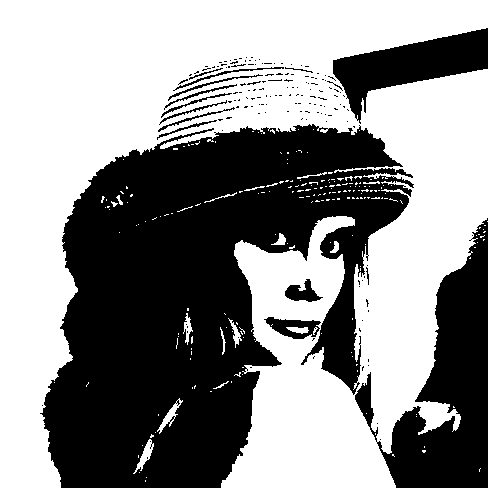
\includegraphics[width=0.3\textwidth]{otsu_custom.png}
  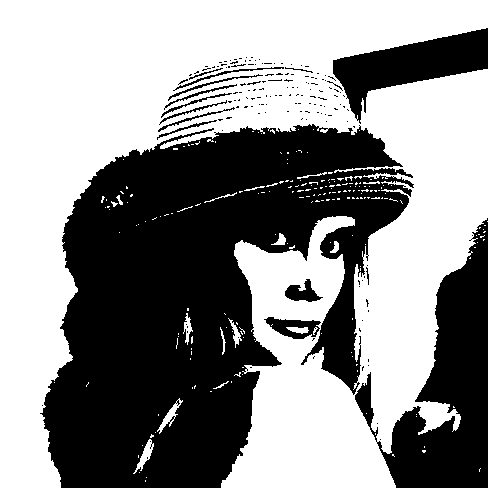
\includegraphics[width=0.3\textwidth]{dilated_image.png}
  \caption{Links: binarisiertes Bild mit Rauschen, Rechts: nach Morphologie}
\end{figure}

\subsection{Aufgabe 4: Kombination mit Originalbild}

Das finale Binärbild wurde als Maske genutzt, um das Originalbild zu filtern. Nur Pixel, die im Binärbild den Wert 1 (weiß) hatten, blieben erhalten. Die übrigen Bereiche wurden schwarz dargestellt.

\begin{figure}[H]
  \centering
  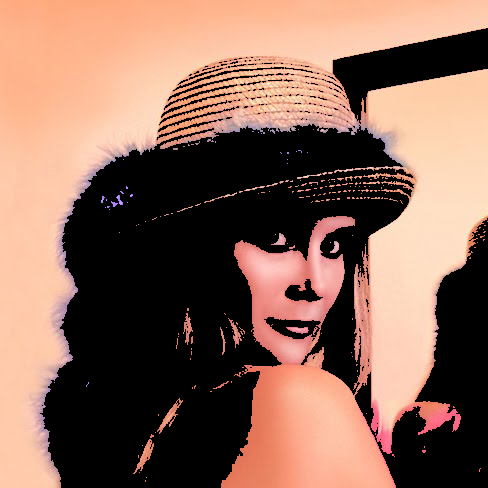
\includegraphics[width=0.4\textwidth]{masked_image.png}
  \caption{Kombination von Originalbild und Binärmaske}
\end{figure}

\section{Zusammenfassung und Ausblick}

In dieser Übung wurden verschiedene Binarisierungsverfahren verglichen und typische Nachbearbeitungsschritte durchgeführt. Das Otsu-Verfahren liefert gute globale Ergebnisse, während das adaptive Thresholding besonders bei inhomogenen Lichtverhältnissen punktet.

Die Kombination mit morphologischen Filtern ermöglichte eine robuste Rauschentfernung. Die Maskierung des Originalbilds stellt eine praxisnahe Anwendung dar, etwa in der Segmentierung relevanter Bildbereiche.

Als nächster Schritt wäre denkbar, weitere Filter wie Median oder Bilateral-Filter zu testen oder die Segmentierung in Richtung Connected Components zu erweitern.

\end{document}